\begin{equation}
    \begin{gathered}
        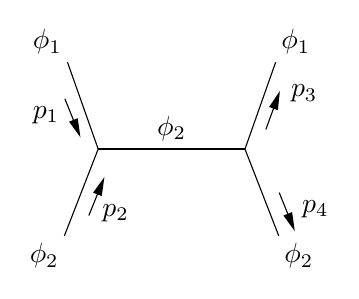
\begin{tikzpicture}[x=0.75pt,y=0.75pt,yscale=-0.75,xscale=0.75]
        %uncomment if require: \path (0,300); %set diagram left start at 0, and has height of 300
        
        %Straight Lines [id:da5433544960650969] 
        \draw    (151.71,99) -- (171.41,154.74) ;
        %Straight Lines [id:da2211889438504424] 
        \draw    (149.71,210.48) -- (171.41,154.74) ;
        %Straight Lines [id:da8914945534164957] 
        \draw    (165.41,197.47) -- (174.66,174.59) ;
        \draw [shift={(175.41,172.74)}, rotate = 472.02] [fill={rgb, 255:red, 0; green, 0; blue, 0 }  ][line width=0.08]  [draw opacity=0] (12,-3) -- (0,0) -- (12,3) -- cycle    ;
        %Straight Lines [id:da8502419018444731] 
        \draw    (150,122.46) -- (159.25,145.33) ;
        \draw [shift={(160,147.18)}, rotate = 247.98000000000002] [fill={rgb, 255:red, 0; green, 0; blue, 0 }  ][line width=0.08]  [draw opacity=0] (12,-3) -- (0,0) -- (12,3) -- cycle    ;
        %Straight Lines [id:da13030876069840058] 
        \draw    (171.41,154.74) -- (265.71,154.74) ;
        %Straight Lines [id:da12916587008636737] 
        \draw    (285.41,99) -- (265.71,154.74) ;
        %Straight Lines [id:da8014677527354779] 
        \draw    (287.41,210.48) -- (265.71,154.74) ;
        %Straight Lines [id:da25455304099872467] 
        \draw    (296.96,205.61) -- (287.71,182.74) ;
        \draw [shift={(297.71,207.47)}, rotate = 247.98] [fill={rgb, 255:red, 0; green, 0; blue, 0 }  ][line width=0.08]  [draw opacity=0] (12,-3) -- (0,0) -- (12,3) -- cycle    ;
        %Straight Lines [id:da09919924539968838] 
        \draw    (287.43,119.33) -- (279.12,142.18) ;
        \draw [shift={(288.12,117.46)}, rotate = 110] [fill={rgb, 255:red, 0; green, 0; blue, 0 }  ][line width=0.08]  [draw opacity=0] (12,-3) -- (0,0) -- (12,3) -- cycle    ;
        
        % Text Node
        \draw (149.71,95.6) node [anchor=south east] [inner sep=0.75pt]    {$\phi _{1}$};
        % Text Node
        \draw (147.71,213.88) node [anchor=north east] [inner sep=0.75pt]    {$\phi _{2}$};
        % Text Node
        \draw (148,125.86) node [anchor=north east] [inner sep=0.75pt]    {$p_{1}$};
        % Text Node
        \draw (172.41,188.5) node [anchor=north west][inner sep=0.75pt]    {$p_{2}$};
        % Text Node
        \draw (218.56,151.34) node [anchor=south] [inner sep=0.75pt]    {$\phi _{2}$};
        % Text Node
        \draw (293.62,126.42) node [anchor=south west] [inner sep=0.75pt]    {$p_{3}$};
        % Text Node
        \draw (300.71,193.1) node [anchor=west] [inner sep=0.75pt]    {$p_{4}$};
        % Text Node
        \draw (287.41,95.6) node [anchor=south west] [inner sep=0.75pt]    {$\phi _{1}$};
        % Text Node
        \draw (289.41,213.88) node [anchor=north west][inner sep=0.75pt]    {$\phi _{2}$};
        \end{tikzpicture}
    \end{gathered} \quad 
    \begin{aligned}[t]
         &\eqqcolon \ii \mathcal{M}_{s2} = \frac{\ii}{(p_1 + p_2)^2 + \ii 0^+} ( \ii \lambda (p_1 + p_2) \cdot p_2) ( \ii \lambda (p_1 + p_2) \cdot p_4) \\
         &= - \ii \frac{\lambda^2 ((p_1 + p_2) \cdot p_2)((p_1 + p_2) \cdot p_4)}{s + \ii 0^+ },
    \end{aligned}
\end{equation}